\section{Plain Transformer}

The \textit{Transformer} \cite{vaswani2017attention} is a \textit{state-of-the-art} architecture proposed by Vaswani et al.
in 2017 in order to overcome the problems encountered by \textit{RNNs} for \textit{Neural Machine Translation} tasks, namely the poor capacities in long-term memory and attention, and the high computational cost.

\begin{figure}[!htb]
    \centering
    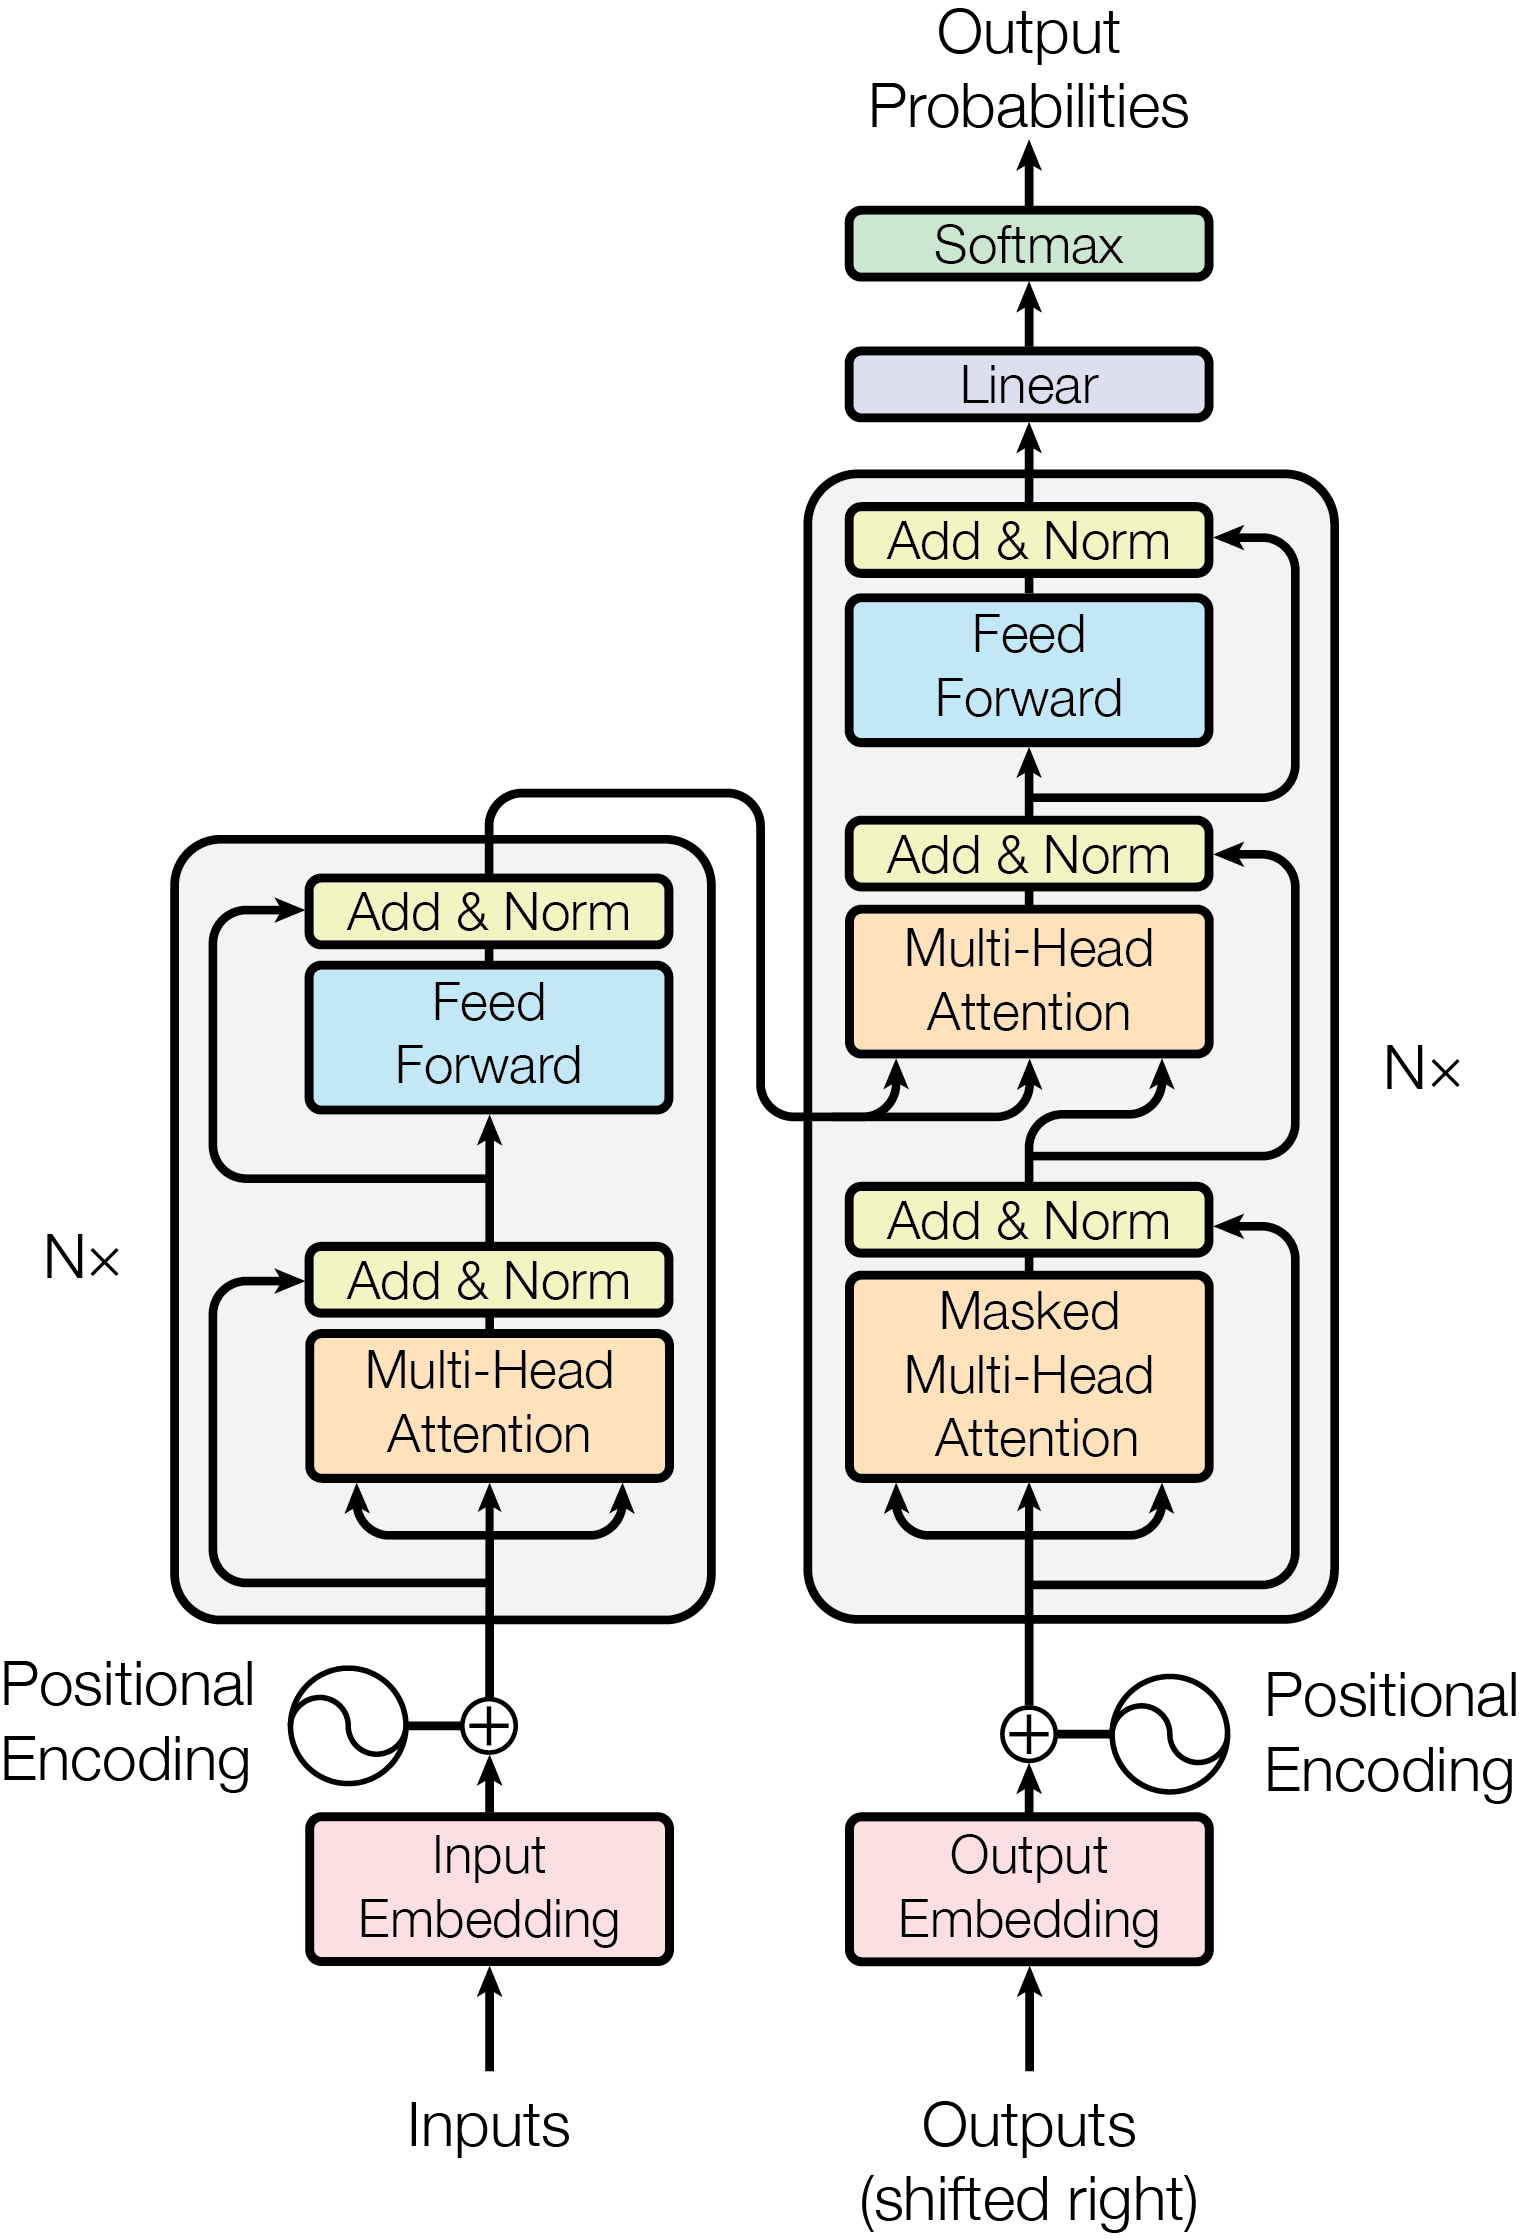
\includegraphics[scale=0.75]{images/model-4_5.png}%
    \caption{Transformer Architecture}%
    \label{transformer}
\end{figure}

As well as standard \textit{Seq2Seq} architectures, the \textit{Transformer} consists of an \texttt{\textsc{Encoder}} and a \texttt{\textsc{Decoder}}, as described in figure \ref{transformer}, both having a number of layers that can be changed in order to have a greater or lower complexity.
Still, differently from previous models, this new one cannot be classified as a recurrent network but it is, instead, a standard feed-forward one, reason why both the \texttt{\textsc{Encoder}}'s and the \texttt{\textsc{Decoder}}'s input tokens must be processed not only with a classical \textsc{Embedding} layer but also with a so-called \textsc{Positional Encoding}, so that the information about the order of the tokens in the sequence is not forgotten even without the presence of recurrent edges.
Finally, these processed inputs are passed through the series of layers, which are made up of two different sub-modules: a \textsc{Multi-Head Attention} (two in the case of the \texttt{\textsc{Decoder}}, as the first one is responsible of processing the decoder input, while the second one is responsible of processing the merged vectors of features extracted both from the encoder input and the decoder input), and a subsequent \textsc{Feed-Forward} block.
Everything is eventually passed through a \textsc{Dense} layer, with softmax activation, to get the output probabilities of each possible token.

The reason why we decided to try this architecture is due to its great ability to generalize in different \textit{Natural Language Processing} tasks as well as its remarkable training speed (being not an \textit{RNN}, it does not suffer the heaviness of backpropagation-through-time).
Furthermore, as we did for the previous models, we decided to start with a simpler version, thus we went back to the standard way of splitting the original text, i.e. with samples of fixed input length and fixed output length, where the output is shifted by one token with respect to the input.

\subsubsection{\textsc{Hyperparameters and Results}}

Though being quite a complex model, the \textit{Transformer} does not have a high number of hyperparameters, which are:
\begin{itemize}
    \item the number of layers for the \texttt{\textsc{Encoder}} and the \texttt{\textsc{Decoder}}
    \item the number of heads for the \textsc{Multi-Head Attention} sub-module
    \item the dimension of all the sub-layers in the model, as well as the \textsc{Embedding} layers, known as \texttt{d\_model}
    \item the inner \textsc{Feed-Forward} layers dimension, known as \texttt{dff}
    \item the dropout rate
\end{itemize}

Overall, this architecture showed a great ability to understand the general structure of the text, as well as our first two models, but in the end nothing more than that could be achieved.
In fact, we could notice a slight increase in the metric for the rhyming scheme, reaching a peak of \textit{0.41} for the \textit{Word-Level} model and \textit{0.44} for the \textit{Subword-Level}, while the score for \texttt{hendecasyllabicness} remained stable for the \textit{Word-Level} and slightly decreased down to a peak of \textit{0.90} for the \textit{Subword-Level} model.